\documentclass[12pt]{article}
\usepackage[T1]{fontenc}
\usepackage[utf8]{inputenc}
\usepackage[polish]{babel}

\usepackage{alltt}
\usepackage{varioref}
\usepackage{enumerate}
\usepackage{amsfonts}
\usepackage{amsmath} 
\usepackage{indentfirst}
\usepackage{graphicx} 
\usepackage{float}
\usepackage{subfig}
\usepackage{listings} 
\usepackage{multirow}
\usepackage{pdfpages}
\usepackage[usenames,dvipsnames,table]{xcolor}
%\usepackage[hdivide={2cm,*,2cm},vdivide={2cm,*,2.5cm}]{geometry}
\frenchspacing

\makeatletter
\def\namedlabel#1#2{\begingroup
   \def\@currentlabel{#2}%
   \label{#1}\endgroup
}
\makeatother
\linespread{1.3}
\usepackage[a4paper, left=2.5cm, right=2.5cm, top=2.5cm, bottom=2.5cm, headsep=1.2cm]{geometry}

% kolory
\usepackage[usenames,dvipsnames]{xcolor}
%Apricot 	Aquamarine 	Bittersweet 	Black
%Blue		BlueGreen 	BlueViolet 	BrickRed
%Brown 		BurntOrange 	CadetBlue 	CarnationPink
%Cerulean 	CornflowerBlue 	Cyan	 	Dandelion
%DarkOrchid 	Emerald 	ForestGreen 	Fuchsia
%Goldenrod 	Gray	 	Green	 	GreenYellow
%JungleGreen 	Lavender 	LimeGreen 	Magenta
%Mahogany 	Maroon	 	Melon	 	MidnightBlue
%Mulberry 	NavyBlue 	OliveGreen 	Orange
%OrangeRed 	Orchid	 	Peach	 	Periwinkle
%PineGreen 	Plum	 	ProcessBlue 	Purple
%RawSienna 	Red	 	RedOrange 	RedViolet
%Rhodamine 	RoyalBlue 	RoyalPurple 	RubineRed
%Salmon 	SeaGreen 	Sepia	 	SkyBlue
%SpringGreen 	Tan	 	TealBlue 	Thistle
%Turquoise 	Violet	 	VioletRed 	White
%WildStrawberry Yellow	 	YellowGreen 	YellowOrange

\usepackage{hyperref} % musi być ostatni!!
\hypersetup{
    bookmarks=true,         % show bookmarks bar?
    pdftoolbar=true,        % show Acrobat's toolbar?
    pdfmenubar=true,        % show Acrobat's menu?
    pdffitwindow=false,     % window fit to page when opened
    pdfstartview={FitH},    % fits the width of the page to the window
    pdfnewwindow=true,      % links in new window
    colorlinks=true,        % false: boxed links; true: colored links
    linkcolor=Black,%MidnightBlue,    % color of internal links
    citecolor=Black,%Plum,        % color of links to bibliography
    filecolor=Black,%magenta,      % color of file links
    urlcolor=Black%cyan           % color of external links
}
%%%%%%%%%%%%%%%%%%%%%%%%%%%%%%%%%%%%%%%%%%%%%%%%%%%%%%%%%%%%%%%%%%%%%%%%%%%%%%%%%%%%%%%%%%%%%%%%%%%%%%%%%%%%%%%%%%%%%%%%%%%%%%%%%%
% początek dokumentu
\begin{document}
\begin{titlepage}
\vspace*{\fill}
 \begin{center}

  \textsc{\LARGE Systemy inteligentnych agentów}\\[2.0cm]
  \textsc{\Large Symulacja rynku spożywczego}\\[1.5cm] 

\vspace*{\fill}
% autorzy:
  \begin{minipage}{0.4\textwidth}
    \begin{flushleft} \large
    \emph{Autorki:}\\
    Weronika Świderska, 233221 \\ Beata Wójciak, 241772
    \end{flushleft}
    \end{minipage}
    \begin{minipage}{0.4\textwidth}
    \begin{flushright} \large
    \emph{Prowadzący:} \\
    Piotr Lipiński
    \end{flushright}
  \end{minipage}

%\vfill
\vspace*{\fill}
% Bottom of the page
{\large \today}
 \end{center}

\end{titlepage}
\newpage
%spis treści
\tableofcontents
\newpage

\section{Wprowadzenie}
Celem naszego projektu było stworzenie systemu inteligentnych agentów, które~---~dzięki wzajemnej komunikacji~---~miały symulować działanie rynku spożywczego.

W~projekcie uwzględniłyśmy kilka różnych typów agentów różniących się zarówno rolami jak i~strategiami.

\section{Opis projektu}
Na naszym rynku działało 6~różnych typów agentów na 3~różnych poziomach:
\begin{itemize}
 \item Poziom~1: agenci, którzy produkują najbardziej podstawowe towary, należą tu:
  \begin{itemize}
  \item Rolnik (produkuje zboże)
  \item Hodowca (produkuje mięso, mleko i~nawóz)
  \item Sadownik (produkuje owoce)
  \end{itemize}
 \item Poziom~2: agenci, którzy kupują towary od agentów 1~poziomu, przetwarzają je, a~następnie sprzedają dalej. Należą tu:
  \begin{itemize}
   \item Piekarz (kupuje zboże, a~sprzedaje pieczywo)
   \item Mleczarz (kupuje mleko, a~sprzedaje produkty mleczne)
  \end{itemize}
 \item Poziom~3: należą tu tylko agenci pełniący rolę klientów, którzy nie produkują żadnych dóbr, a~jedynie kupują je od innych
\end{itemize}

Zależności między agentami przedstawia Rysunek \ref{fig:schemat zależności}.
\begin{figure} [H]
 \centering
 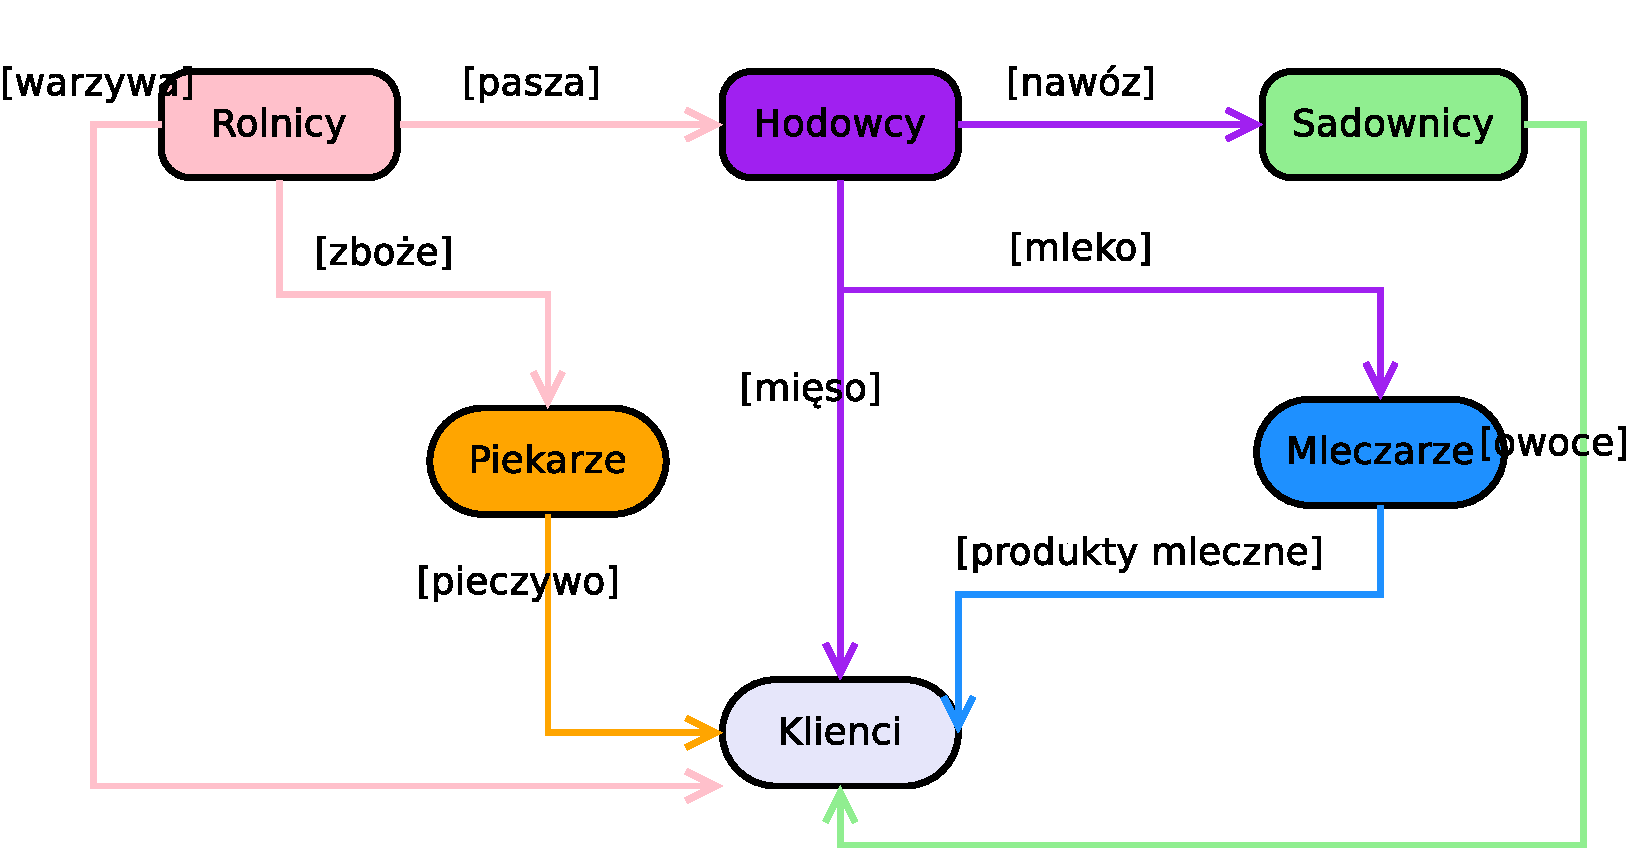
\includegraphics[width=0.8\textwidth]{diagram_kolorowy}
 \caption{Schemat zależności między agentami}
 \label{fig:schemat zależności}
\end{figure}

Na początku każdy agent dostaje pewną ilość dóbr, które może zużyć na handel lub wytworzenie większej ilości produktów (np. obsiać pole). Wielkość początkowych zasobów agenta ma wpływ na to, jak radzi on sobie
na rynku~---~szczegółowe wyniki z tym związane przedstawione zostały w Rozdziale~\ref{chapter: rezultaty}.

\section{Architektura systemu}
Program został napisany w~Javie z~wykorzystaniem JADE. Ułatwiło to znacznie implementację komunikacji między agentami zgodnie ze standardami FIPA.

\section{Komunikacja między agentami}
Komunikacja między agentami odbywa się w~kilku etapach. W~każdym etapie muszą być przeprowadzone pewne akcje, które następnie są komunikowane drugiej stronie.

Podczas dokonywania transakcji
można wyróżnić następujące etapy (schemat komunikacji przedstawia Rysunek~\ref{fig:schemat komunikacji}):
\begin{enumerate}
 \item Na początku każdego tygodnia każdy agent, który sprzedaje jakiś produkt informuje potencjalnych kupców co sprzedaje, w~jakiej cenie i~w~jakiej ilości. Wysyła to za pomocą komunikatu typu \verb INFORM .
 \item Po otrzymaniu ofert od wszystkich sprzedających oferujących dobro poszukiwane przez kupca, podejmuje on decyzję, na które oferty się może przystać i~na jakich warunkach (może zaoferować inną cenę i~ilość niż sprzedający).
 \item Kupujący odsyła sprzedającemu swoje propozycje (lub pustą wiadomość, by dać znać, że nie jest zainteresowany daną ofertą) używając komunikatu typu \verb CFP .
 \item Po otrzymaniu propozycji od wszystkich kupujących, do których sprzedający wysłał wiadomość sprzedający analizuje oferty i~podejmuje ostateczną decyzję co do tego, na jakie transakcje przystaje. 
Wysyła klientom swoje decyzje korzystając z~komunikatu typu \verb PROPOSE .
 \item Klient po otrzymaniu i~analizie decyzji od sprzedającego akceptuje ją lub odrzuca, o~czym informuje sprzedającego komunikatem typu \verb ACCEPT_PROPOSAL \newline albo \verb REJECT_PROPOSAL .
 \item Jeśli sprzedawca otrzymał zgodę kupującego na transakcję, to sprawdza, czy może ona wciąż być zrealizowana (czy w~międzyczasie towary nie zostały sprzedane komuś innemu).
Jeśli wszystko jest w~porządku potwierdza klientowi wykonanie transakcji komunikatem typu \verb CONFIRM  i~aktualizuje stan posiadanych produktów. W~przeciwnym razie wysyła komunikat typu \verb REFUSE .
 \item Po otrzymaniu potwierdzenia wykonania transakcji kupujący również uaktualnia zawartość swoich magazynów.
\end{enumerate}

\begin{figure} [H]
 \centering
 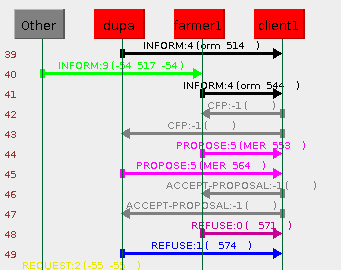
\includegraphics[width=0.8\textwidth]{schemat_komunikacji_v1}
 \caption{Schemat komunikacji między agentami}
 \label{fig:schemat komunikacji}
\end{figure}

\section{Zaimplementowane strategie kupujące agentów}
\begin{enumerate}
 \item \textbf{Strategia naiwna}: Agent wybiera zawsze najtańszą ofertę.
  \begin{itemize}
  \item \textbf{Prosta}: Agent kupuje od sprzedającego z~najtańszą ofertą tyle ile potrzebuje, a~jeśli to jest mniej niż potrzebuje to nic nie robi więcej.
  \item \textbf{Złożona}: Jeśli agent oferujący najtańszą ofertę nie ma wystarczająco dużo towaru, to pozostały potrzebny towar bierze od agenta z~drugą w kolejności ceną itd.
  \end{itemize}
 \item \textbf{Strategia mniej naiwna}: Agent kupuje od najtańszego tyle ile może, a~kolejnym w~kolejności oferuje cenę najniższej oferty.
 \item Oferuje cenę najniższej oferty temu, który ma tyle, ile on potrzebuje.
 \item Jeśli ceny są niższe niż w poprzednich tygodniach to kupuje więcej (proporcjonalnie do różnicy cen), a jeśli są wyższe - to mniej
\end{enumerate}

\section{Zaimplementowane strategie kupujące agentów}
\begin{enumerate}
 \item Akceptuje tylko oferty nie wyższe niż jego własne
 \item Akceptuje oferty niższe o nie więcej niż 10\% jego
 \item Akceptuje losowo (np. z prawdopodobieństwem 40\%)
 \item Jeśli ceny są wyższe niż w poprzednich tygodniach to sprzedaje więcej.
\end{enumerate}


\section{Otrzymane rezultaty}\label{chapter: rezultaty}
tu będą wykresy
\section{Wnioski i~podsumowanie}
\end{document}
